% Archetype F2 : diagramme de flux des donnees (CONSORT genomique)
% Repond a la seule question que tout relecteur pose : comment passe-t-on de
% N genomes publics a n genomes analyses, et qu'est-ce qui est tombe a chaque cran ?
\documentclass[border=4pt]{standalone}
\usepackage[T1]{fontenc}
\usepackage{lmodern}
\usepackage{xcolor}
\usepackage{tikz}
\usetikzlibrary{positioning,arrows.meta,calc,fit,backgrounds}

\definecolor{keepblue}{HTML}{0072B2}
\definecolor{dropred}{HTML}{D55E00}
\definecolor{neutralgrey}{HTML}{4D4D4D}
\definecolor{stagetint}{HTML}{EAF2F8}
\definecolor{droptint}{HTML}{FBEEE6}

\begin{document}
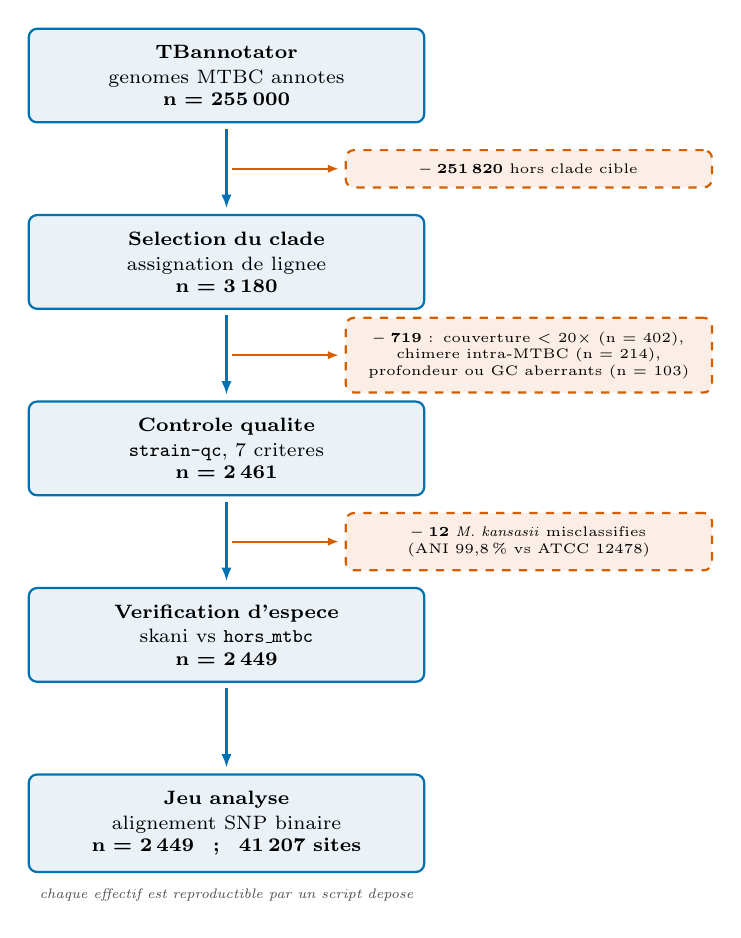
\begin{tikzpicture}[
    every node/.style={font=\scriptsize, align=center},
    stage/.style={
      draw=keepblue, thick, rounded corners=3pt, inner sep=6pt,
      text width=4.6cm, fill=stagetint, font=\scriptsize
    },
    drop/.style={
      draw=dropred, thick, dashed, rounded corners=3pt, inner sep=5pt,
      text width=4.3cm, fill=droptint, font=\tiny
    },
    flow/.style={-{Latex[length=5pt]}, line width=1pt, keepblue, shorten >=2pt, shorten <=2pt},
    excl/.style={-{Latex[length=4pt]}, line width=0.8pt, dropred, shorten >=2pt, shorten <=2pt},
    tag/.style={font=\tiny\itshape, text=neutralgrey}
  ]

  \node[stage] (src) {\textbf{TBannotator}\\[1pt] genomes MTBC annotes\\ \textbf{n = 255\,000}};
  \node[stage, below=1.15cm of src] (sel) {\textbf{Selection du clade}\\[1pt] assignation de lignee\\ \textbf{n = 3\,180}};
  \node[stage, below=1.15cm of sel] (qc)  {\textbf{Controle qualite}\\[1pt] \texttt{strain-qc}, 7 criteres\\ \textbf{n = 2\,461}};
  \node[stage, below=1.15cm of qc]  (spe) {\textbf{Verification d'espece}\\[1pt] skani vs \texttt{hors\_mtbc}\\ \textbf{n = 2\,449}};
  \node[stage, below=1.15cm of spe] (fin) {\textbf{Jeu analyse}\\[1pt] alignement SNP binaire\\ \textbf{n = 2\,449 \, ; \, 41\,207 sites}};

  \foreach \a/\b in {src/sel, sel/qc, qc/spe, spe/fin} {\draw[flow] (\a) -- (\b);}

  % Les exclusions se chiffrent et se motivent, une par une : c'est la moitie
  % de l'information du diagramme, pas une annexe.
  \node[drop, right=1.5cm of $(src)!0.5!(sel)$] (d1)
    {\textbf{-- 251\,820} hors clade cible};
  \node[drop, right=1.5cm of $(sel)!0.5!(qc)$] (d2)
    {\textbf{-- 719} : couverture $<$ 20$\times$ (n = 402),\\ chimere intra-MTBC (n = 214),\\ profondeur ou GC aberrants (n = 103)};
  \node[drop, right=1.5cm of $(qc)!0.5!(spe)$] (d3)
    {\textbf{-- 12} \emph{M. kansasii} misclassifies\\ (ANI 99{,}8\,\% vs ATCC 12478)};

  \foreach \d/\a/\b in {d1/src/sel, d2/sel/qc, d3/qc/spe}
    {\draw[excl] ($(\a)!0.5!(\b)$) -- (\d.west);}

  \node[tag, below=2pt of fin] {chaque effectif est reproductible par un script depose};

\end{tikzpicture}
\end{document}
